This section describes firsty what a data storage is and which typologies of storages exist. Thus this project's data storage layer, \gls{HopsFS}, is presented, starting from its evolution from \gls{HDFS}, going in the details about its tools, and ending with possible alternatives, the cloud object storages.

\subsection{Block storage vs. File storage vs. Object storage}
\label{subsec:block_vs_file_vs_object}

Data can be stored and organized in physical storages, such as \glspl{HDD} or \glspl{SSD}. The three main type of data storage are (1)~Block storage, (2)~File storage, and (3)~Object storage briefly compared in Table \ref{tab:short_storage_comparison}. Each typology is describe in the following paragraphs, and their pros and cons are summarized in Table \ref{tab:long_storage_comparison}. This subsection is a re-elaboration of three articles from major cloud providers (Amazon, Google, and IBM) \cite{BlockVsFile, HowObjectVs, ObjectVsFile2021} according to the author's understanding.

\begin{table}[!ht]
    \begin{center}
      \caption[Data storage features comparison]{Data storage features comparison. Table inspired by major cloud providers articles \cite{BlockVsFile,HowObjectVs,ObjectVsFile2021}.}
      \label{tab:short_storage_comparison}
      \begin{tabular}{cccc}
        \toprule
        \textbf{Characteristics} & \textbf{Block Storage} & \textbf{File Storage} & \textbf{Object Storage}\\
        \midrule
        Performance & High & High & Low\\
        Scalability & Low & Low & High\\
        Cost & High & High & Low\\
        \bottomrule
      \end{tabular}
    \end{center}
\end{table}

\subsubsection*{Block Storage}

Block storage is a data storage method that divides data into discrete blocks of fixed size, each assigned a unique identifier. These blocks are stored independently on a storage system, such as a \gls{SAN} or within a cloud environment. 

This decentralized approach offers several key advantages. Firstly, it enables high performance with fast read/write speeds and low latency, crucial for demanding applications like databases and virtual machine environments. Secondly, block storage provides direct, low-level access to storage volumes, similar to physical disks, granting users and applications granular control over data organization and management. This flexibility allows for a wide range of use cases, including powering virtual machine environments, supporting high-performance databases, and enabling efficient file sharing.

While offering significant benefits, block storage also presents certain limitations. It typically requires specialized hardware and infrastructure, potentially leading to higher costs compared to other storage options. Furthermore, while it offers a degree of scalability, expanding beyond certain limits can become complex and costly. Despite these considerations, block storage remains a vital technology for modern IT environments, enabling high performance, flexibility, and agility in data management.

\subsubsection*{File Storage}

File storage is a hierarchical data organization method that stores data in files, which are organized into folders within a structure of directories and subdirectories. Files are characterized by extensions (e.g., ".txt", ".png", ".csv"), defining how the data is organized and accessed. This system simplifies locating and retrieving individual files when their exact paths are known, making it intuitive and user-friendly.

This structure is particularly beneficial for managing structured data and is widely used in \gls{PC} and \gls{NAS} devices. It enables centralized file sharing on  \gls{LAN} and supports common file-level protocols, ensuring compatibility across Windows and Linux systems. Storing data on a separate NAS device or in the cloud also enhances data protection and disaster recovery, with options to replicate data across multiple geographic locations for added security.

However, as the volume of files grows, scaling becomes challenging. Locating files in a large hierarchy can be time-consuming, and scaling often requires investing in additional or higher-capacity hardware. Cloud-based file storage services mitigate these challenges by offering scalable, off-site storage managed by service providers. These services eliminate hardware maintenance costs and provide flexible, subscription-based models that adapt to varying storage and performance needs.

File storage remains popular for applications requiring simplicity and centralized access, such as file sharing, personal storage, and cloud-based platforms like Dropbox and Google Drive. While other storage solutions may be better suited for managing massive datasets or unstructured data, file storage's accessibility, affordability, and ease of use ensure its ongoing relevance.

\subsubsection*{Object Storage}

Object storage is a flat data storage method that organizes data into self-contained objects, each containing metadata that describes attributes like size, creation date, and unique identifiers. This metadata not only defines the data but also enables efficient querying and retrieval of large datasets. This makes object storage particularly well-suited for managing unstructured data, such as videos, images, and other media files that do not fit neatly into traditional hierarchical systems.

The flat structure of object storage eliminates complex hierarchies like folders and directories, simplifying organization and improving scalability. This structure allows object storage systems to replicate data across multiple regions, enhancing accessibility and fault tolerance in case of hardware failures. As a result, users benefit from faster data access in different parts of the world and robust disaster recovery options.

However, object storage has limitations. Objects are immutable, meaning they cannot be directly altered once created. Any changes require the creation of a new object. Additionally, object storage does not support transactional operations, as it lacks mechanisms like file locking, making it unsuitable for applications requiring frequent updates or real-time data changes. It also has slower writing performance compared to file or block storage solutions.

Overall, object storage is an excellent choice for use cases requiring high scalability, such as social networks, video streaming platforms, and cloud-based services. Its flat structure and metadata-driven design are ideal for managing large, static datasets. However, other storage options are preferred when high performance is required for frequently changing files or when transactional consistency is critical.

\begin{table}[h!]
    \centering
    \caption[Data storage pros and cons comparison]{Data storage pros and cons comparison. Table inspired by major cloud providers articles \cite{BlockVsFile,HowObjectVs,ObjectVsFile2021}.}
    \label{tab:long_storage_comparison}
    \begin{tabular}{|p{1.8cm}|p{4.8cm}|p{5.3cm}|}
        \hline
        \textbf{Storage Typology} & \textbf{Pros} & \textbf{Cons} \\
        \hline
        Block & 
        \begin{tabular}[t]{@{}l@{}}
            High performance \\ 
            High reliability \\ 
            Easy updates
        \end{tabular} & 
        \begin{tabular}[t]{@{}l@{}}
            Lacks metadata \\ 
            Not easily searchable \\ 
            High cost
        \end{tabular} \\
        \hline
        File & 
        \begin{tabular}[t]{@{}l@{}}
            Easy on small-scale \\ 
            User-friendly \\ 
            User-manageable \\ 
            File-level locking
        \end{tabular} & 
        \begin{tabular}[t]{@{}l@{}}
            Inefficient on unstructured data \\ 
            Limited scalability
        \end{tabular} \\
        \hline
        Object & 
        \begin{tabular}[t]{@{}l@{}}
            Ideal on unstructured data \\ 
            Cost-effective \\ 
            Highly scalable \\ 
            Efficient advanced retrieval \\ 
        \end{tabular} & 
        \begin{tabular}[t]{@{}l@{}}
            No file-level locking \\ 
            Low performance \\ 
            No data updates
        \end{tabular} \\
        \hline
    \end{tabular}
\end{table}

\subsection{\glsfmtlong{HDFS}}
% Restart from
Prova prova

Figure \ref{fig:hdfs_schema} presents a simplified visual representation of the Namenode and Datanodes basic operations in \gls{HDFS}.

\begin{figure}[!ht]
    \begin{center}
      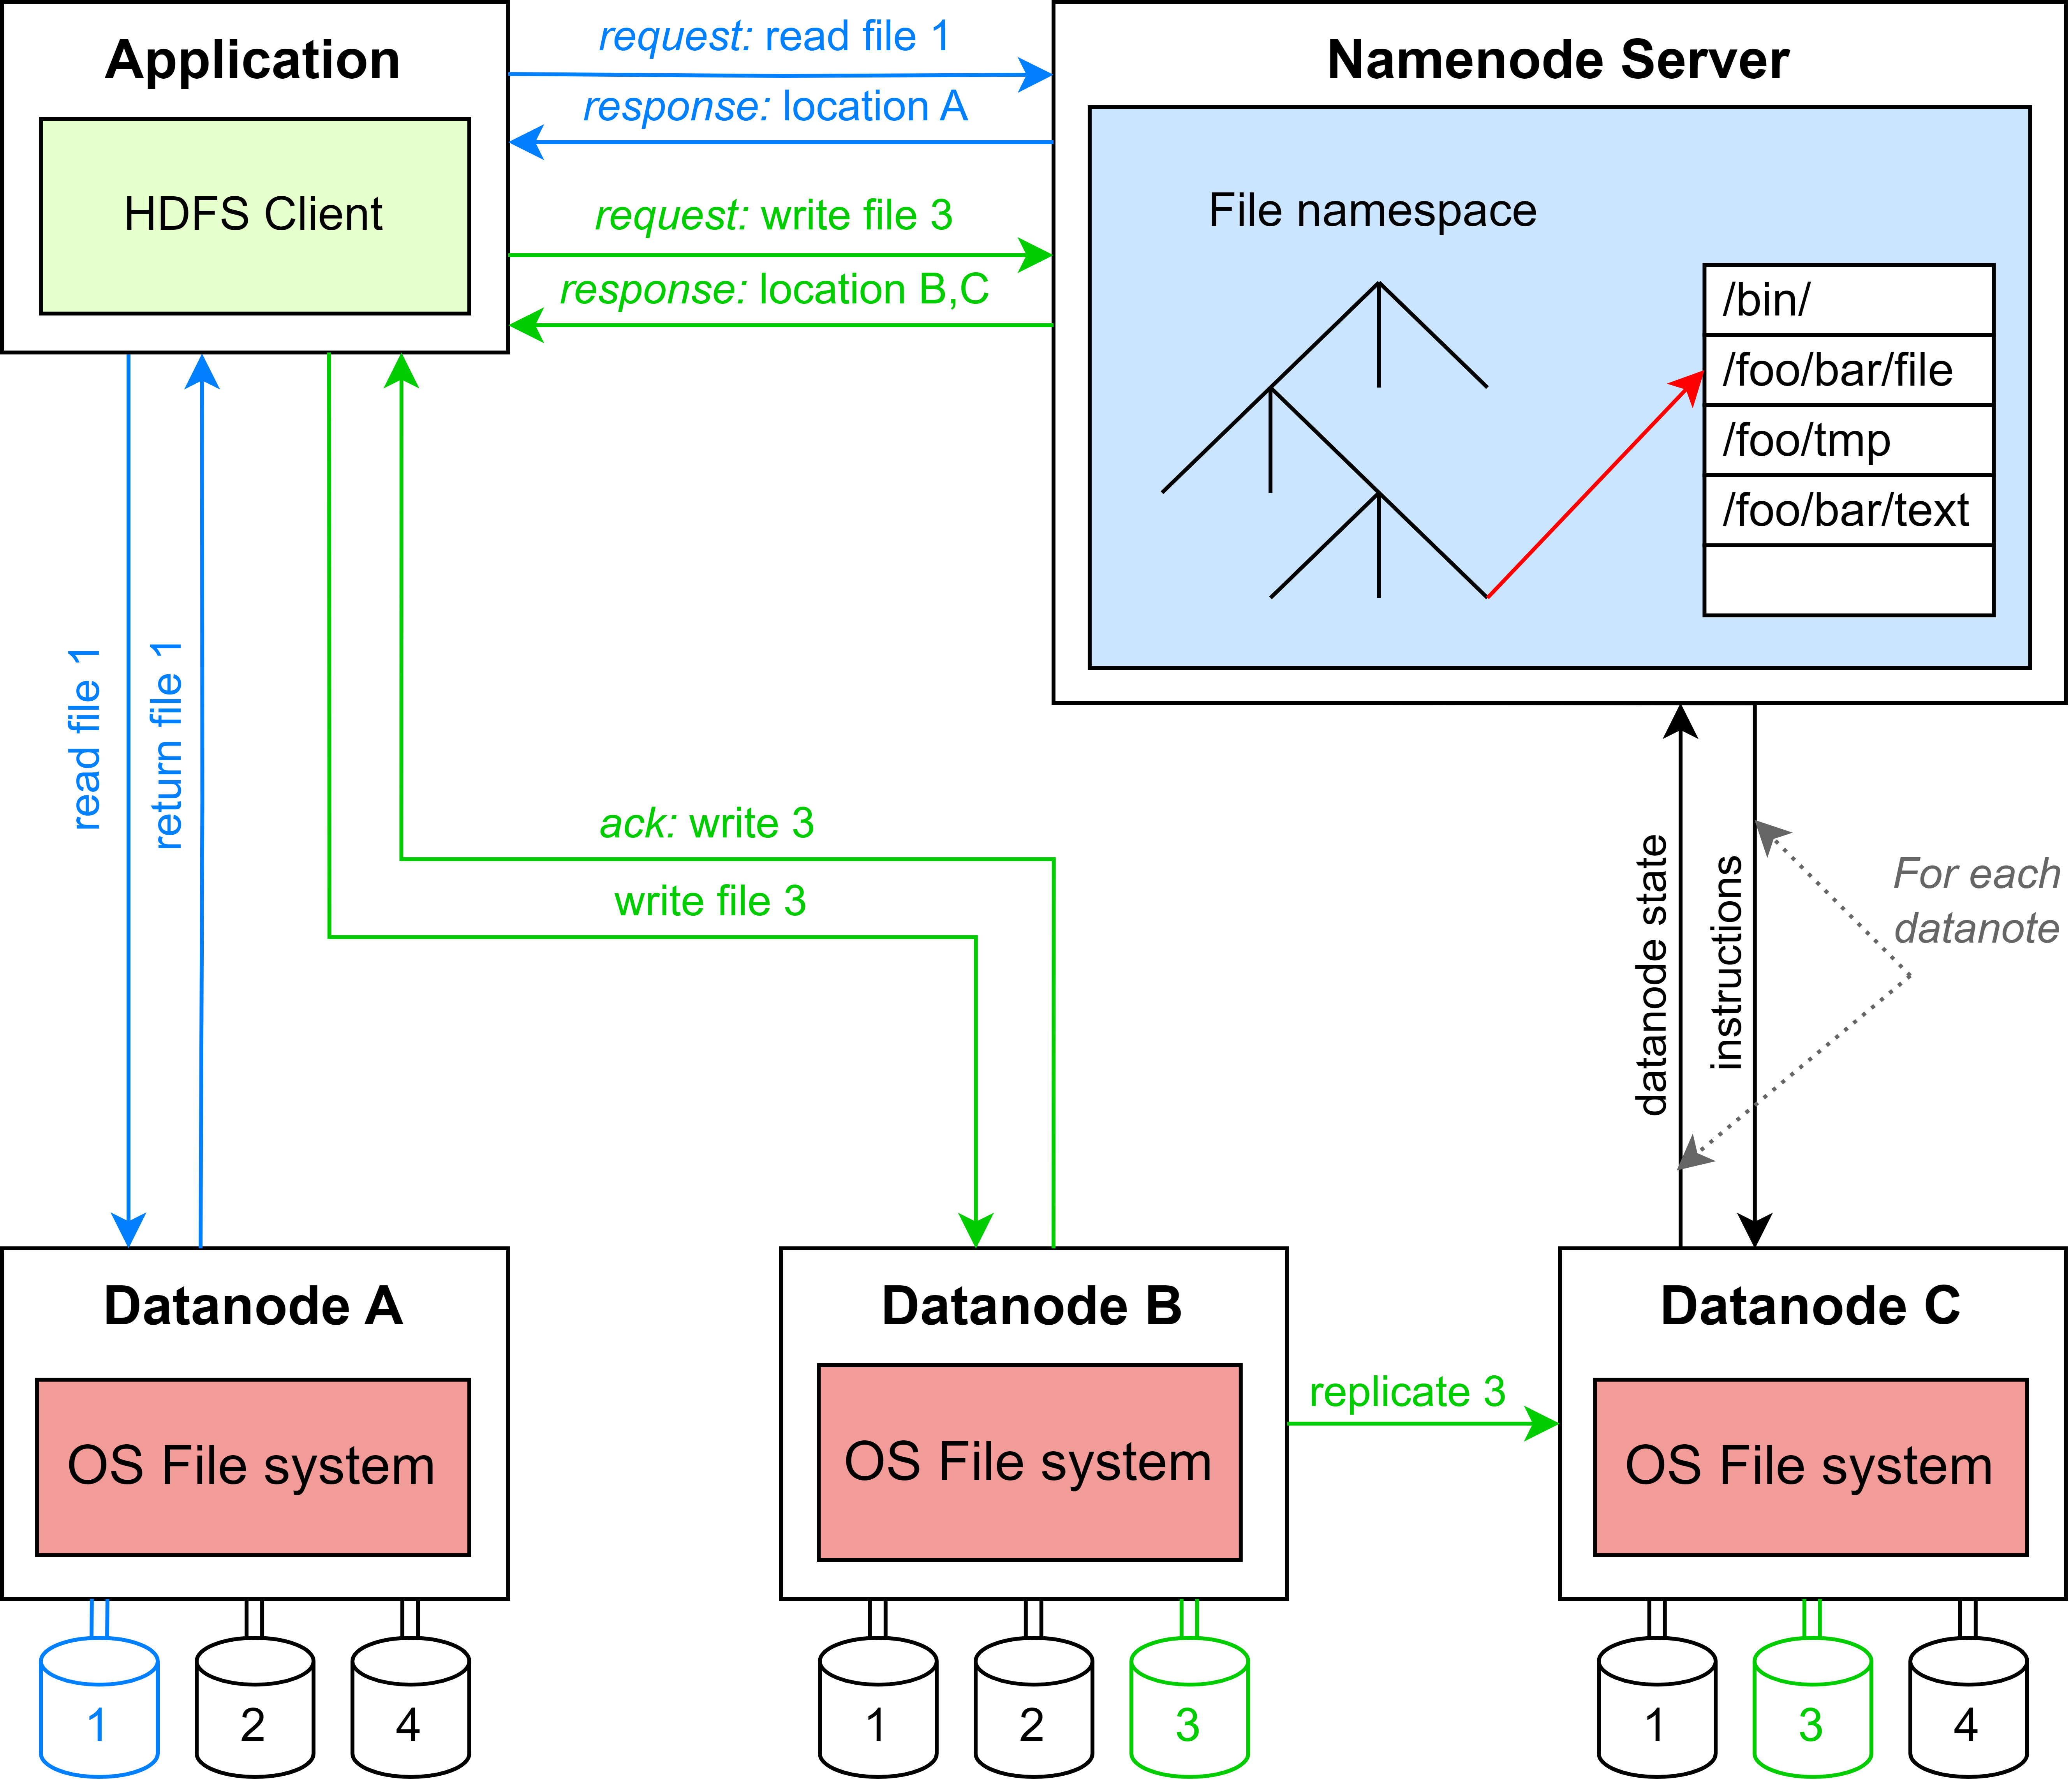
\includegraphics[width=\textwidth]{figures/2-background_and_related_work/hdfs_schema.png}
    \end{center}
    \caption[Hadoop Distributed File System architecture]{\glsentryfull{HDFS} architecture displaying in different colors basic operations: read (blue), write (green) and Namenode-Datanodes management messages (black). Note: for representation simplicity, files are not segmented into blocks and a single Namenode-Datanode message exchange is pictured. Diagram inspired by the Data-intensive Computing lectures at KTH by Prof. A. H. Payberah. Course website available at \url{https://www.kth.se/student/kurser/kurs/ID2221?l=en}.}
    \label{fig:hdfs_schema}
\end{figure}

\subsection{\glsfmtshort{HopsFS}}

\subsection{Cloud object stores, an alternative}
